\chapter{Architettura software}


\section{Architettura generale}

Il progetto è stato realizzato seguendo un'architettura software client-server (figura \ref{fig:arch}). In questa architettura i componenti principali sono: il client rappresentato dall'applicazione iPad oggetto di questo documento, e il lato server scomposto in \emph{middleware} e i sistemi messi a disposizione dal cliente (l'istituto bancario).

Il middleware opera da intermediario tra i servizi bancari e l'applicazione. Tale componente ha il compito di ricevere le richieste dal client, di sottomettere a sua volta queste richieste ai servizi lato banca e di ritornare i dati al client opportunamente formattati.

Le richieste verso il middleware (ospitante un webserver \emph{Apache}) vengono eseguite seguendo un'architettura \emph{RESTFUL}  che prevede richieste \emph{HTTP} (POST, GET, PUT, DELETE). Le risposte fornite dal middleware verso il client sono costruite in formato \emph{JSON}.


\begin{figure}[!htbp]
\centering
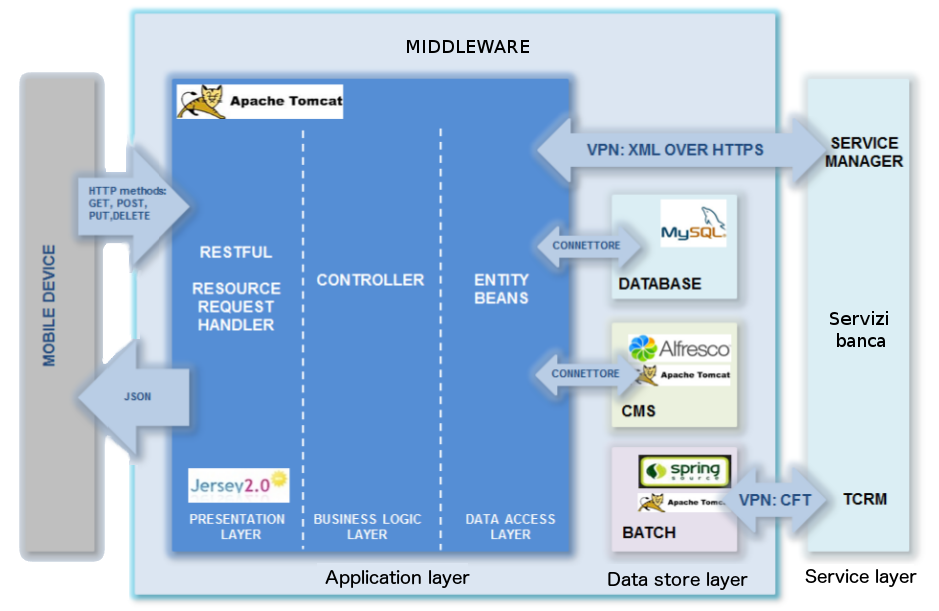
\includegraphics[scale=0.60]{architettura/architect.png}
\caption{Architettura client-server}
\label{fig:arch}
\end{figure}


\section{Architettura applicazione}

L'applicazione è stata progettata usando il design pattern \emph{MVC} (Model-View-Controller, figura \ref{fig:mvc}). In tale pattern ogni oggetto dell'applicazione assolve uno dei seguenti ruoli:
\begin{itemize}
 \item Model: gli oggetti di tipo model hanno il compito di incapsulare i dati specifici a un'applicazione e di definire le logiche per modificare e processare tali dati
 \item View: sono gli oggetti dell'applicazione visibili all'utente. Tali oggetti hanno il compito di visualizzare i dati dell'applicazione e di permetterne l'interazione (esempio la modifica)
 \item Controller: è un oggetto che opera da intermediario tra la view e uno o più model dell'applicazione. Tali oggetti hanno quindi la funzione di comunicare i cambiamenti tra le view e i model, e viceversa.
\end{itemize}

L'utilizzo del pattern MVC permette una migliore estensione del codice, di costruire componenti riusabili e migliorare la definizione delle interfacce.

\begin{figure}[!htbp]
\centering
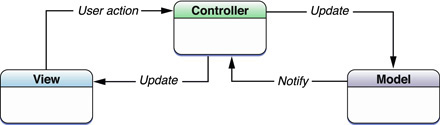
\includegraphics[scale=0.70]{architettura/mvc.png}
\caption{Schema del pattern MVC}
\label{fig:mvc}
\end{figure}

Nei prossimi paragrafi verranno descritte le classi principali del progetto.

\section{Diagramma delle classi}

\subsection{Connessione ai servizi}
La parte relativa alla gestione delle chiamate ai servizi è stata realizzata implementando delle classi \emph{singleton}. Tali classi estendono la libreria di terze parti \texttt{AFNetworking} che opera da wrapper sulle tecnologie di comunicazione messe a disposizione dall'SDK iOS (Foundation URL Loading System). 

Utilizzare una libreria coome AFNetworking ha permesso di ridurre i tempi di sviluppo e di sfruttare le potenzialità offerte dalle sue API come: la serializzazione e deserializzazione dei dati, la possibilità di effettuare richieste HTTP asincrone, una gestione efficiente delle code, la gestione di sessioni, ecc\dots.  

\begin{figure}[!htbp]
\centering
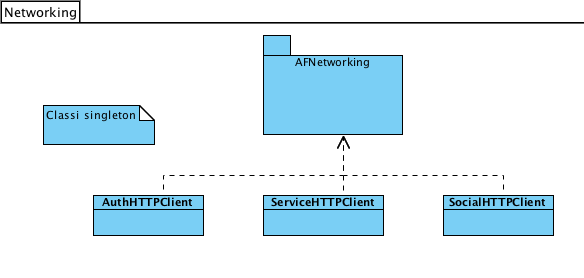
\includegraphics[scale=0.70]{architettura/networkingClass.png}
\caption{Diagramma delle classi per le connessioni di rete}
\end{figure}

% i servizi sono separati da quelli di autenticazione perchè gli  standard oauth richiedono la separazione i sottodimini diversi.

\subsection{Caching dei dati}
Per migliorare le prestazioni e limitare il traffico di rete generato durante l'utilizzo dell'applicazione è stato implementato un meccanismo di caching dei dati che consente di salvare in memoria primaria i dati necessari all'applicazione durante una sessione di utilizzo. 

\begin{figure}[!htbp]
\centering
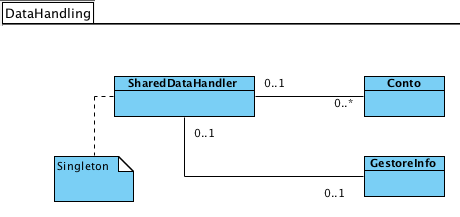
\includegraphics[scale=0.70]{architettura/cacheClass.png}
\caption{Diagramma delle classi per il caching dei dati}
\end{figure}

\subsection{Autenticazione e sicurezza dei dati}

Uno degli aspetti fondamentali considerati durante la progettazione  